\documentclass[a4paper,11pt]{article}
\title{PAG Static \& Dynamic Analysis of Spring Constant}
\author{Izaak van Dongen}

% make the document take up more of the page
\usepackage[margin=1in,headheight=13.6pt]{geometry}

% so the title can be accessed by fancyhdr (and is automatically correctly
% spelled etc)
\makeatletter
\let\thetitle\@title
\makeatother

% custom document header/footer
\usepackage{fancyhdr}
\usepackage{lastpage}

\pagestyle{fancy}
\fancyhf{}
\lhead{\thetitle}
\rhead{Izaak van Dongen}
\rfoot{Page \thepage\ of \pageref{LastPage}}

%% fonts
%\usepackage[p,osf]{cochineal}
%\usepackage[scale=.95,type1]{cabin}
%\usepackage[cochineal,bigdelims,cmintegrals,vvarbb]{newtxmath}
%% fixed width font with 80 chars per listing line
%\usepackage[scaled=.94]{newtxtt}
%\usepackage[cal=boondoxo]{mathalfa}
\usepackage{amsfonts}

% maths symbols and other stuff (supersedes the ams* packages)
\usepackage{mathtools}

% for typesetting differentials
\usepackage{commath}

% no paragraph indent
\usepackage[parfill]{parskip}

% pretty table rules and multirow entries. Also page-breaking tables
\usepackage{booktabs}
\usepackage{multirow}
\usepackage{longtable}

% plotting mathematical functions (needs version request)
\usepackage{pgfplots}
\pgfplotsset{compat=1.15}

% \url function and clickable table of contents. no ugly red boxes though
\usepackage[hidelinks]{hyperref}

% For framing definitions
\usepackage[framemethod=tikz]{mdframed}
\usepackage[most]{tcolorbox}

\newtcolorbox{definition}{
freelance,
before=\par\vspace{2\bigskipamount}\noindent,
after=\par\bigskip,
frame code={
  \node[
  anchor=south west,
  inner xsep=8pt,
  xshift=8pt,
  rounded corners=5pt,
  font=\bfseries\color{white},
  fill=gray] at (frame.north west) (tit) {\strut Definition:};
  \draw[
  line width=3pt,
  rounded corners=5pt,gray
  ] (tit.west) -| (frame.south west) -- ([xshift=15pt]frame.south west);
},
interior code={},
top=2pt
}

% for better table of contents stuff, providing the \listof* commands and not
% listing the tables in the table of contents
\usepackage[nottoc,notlof,notlot]{tocbibind}

% more advanced handling of utf8 and fonts or something. apparently good to have
\usepackage[utf8]{inputenc}
\usepackage[T1]{fontenc}

% somehow this fixes ~ signs in listing environments
\usepackage{lmodern}

% bibliography management with square braces for citations
\usepackage[square,numbers]{natbib}

% graphics, like eps files and stuff (supersedes graphics)
\usepackage{graphicx}

% used to horizontally align floats
\usepackage{subfig}

% used for figures
\usepackage{float}

% needed for colouring and stuff (xcolor supersedes color)
\usepackage{xcolor}

\definecolor{codegreen}{rgb}{ 0,0.6,0}

% listings of code
\usepackage{minted}
\setminted{breaklines,
           breakbytokenanywhere,
           linenos
}
\usemintedstyle{friendly}
% bigger line numbers
\renewcommand\theFancyVerbLine{\footnotesize\arabic{FancyVerbLine}}

% that can break across pages while being captioned figures
\usepackage{caption}
\newenvironment{longlisting}
{\addvspace{\baselineskip}\captionsetup{type=listing}}
{\addvspace{\baselineskip}}

% allow maths to break across pages
\allowdisplaybreaks

\usepackage[separate-uncertainty]{siunitx}

\begin{document}
    \maketitle%\thispagestyle{empty} % no page number under title

\begin{longlisting}
\inputminted{R}{analyse.r}
\caption{R source}
\end{longlisting}

\begin{longlisting}
\begin{minted}{text}
    m    x1    x2    x3    x4    x5      x        F
1 0.1 0.585 0.586 0.587 0.587 0.588 0.5866 0.980665
2 0.2 0.625 0.626 0.625 0.628 0.627 0.6262 1.961330
3 0.3 0.663 0.665 0.664 0.665 0.664 0.6642 2.941995
4 0.4 0.702 0.704 0.701 0.704 0.704 0.7030 3.922660
5 0.5 0.741 0.742 0.739 0.742 0.739 0.7406 4.903325
6 0.6 0.776 0.777 0.775 0.776 0.780 0.7768 5.883990

Call:
lm(formula = F ~ x, data = static_df)

Residuals:
        1         2         3         4         5         6
 0.027502 -0.011303 -0.008916 -0.027125 -0.014441  0.034284

Coefficients:
            Estimate Std. Error t value Pr(>|t|)
(Intercept) -14.1484     0.1195  -118.4 3.06e-08 ***
x            25.7442     0.1742   147.7 1.26e-08 ***
---
Signif. codes:  0 ‘***’ 0.001 ‘**’ 0.01 ‘*’ 0.05 ‘.’ 0.1 ‘ ’ 1

Residual standard error: 0.02776 on 4 degrees of freedom
Multiple R-squared:  0.9998,	Adjusted R-squared:  0.9998
F-statistic: 2.183e+04 on 1 and 4 DF,  p-value: 1.259e-08

    m    T1    T2    T3    T4    T5      T    plot_y    plot_x
1 0.1  7.61  7.90  8.15  8.22  8.23 0.4011 245.38862 10.000000
2 0.2 11.54 11.24 11.16 11.31 11.23 0.5648 123.75717  5.000000
3 0.3 13.42 13.64 13.68 13.40 13.53 0.6767  86.21193  3.333333
4 0.4 15.71 15.69 15.50 15.55 15.52 0.7797  64.93886  2.500000
5 0.5 17.33 17.42 17.31 17.19 17.26 0.8651  52.75056  2.000000
6 0.6 18.63 18.64 18.60 18.69 18.88 0.9344  45.21620  1.666667

Call:
lm(formula = plot_y ~ plot_x, data = dynamic_df)

Residuals:
      1       2       3       4       5       6
 0.3031 -1.2932  1.1733 -0.0939 -0.2787  0.1893

Coefficients:
            Estimate Std. Error t value Pr(>|t|)
(Intercept)   5.0152     0.6427   7.804  0.00145 **
plot_x       24.0070     0.1289 186.242 4.99e-09 ***
---
Signif. codes:  0 ‘***’ 0.001 ‘**’ 0.01 ‘*’ 0.05 ‘.’ 0.1 ‘ ’ 1

Residual standard error: 0.9032 on 4 degrees of freedom
Multiple R-squared:  0.9999,	Adjusted R-squared:  0.9999
F-statistic: 3.469e+04 on 1 and 4 DF,  p-value: 4.986e-09
\end{minted}
\caption{Model results}
\end{longlisting}

\begin{figure}[H]
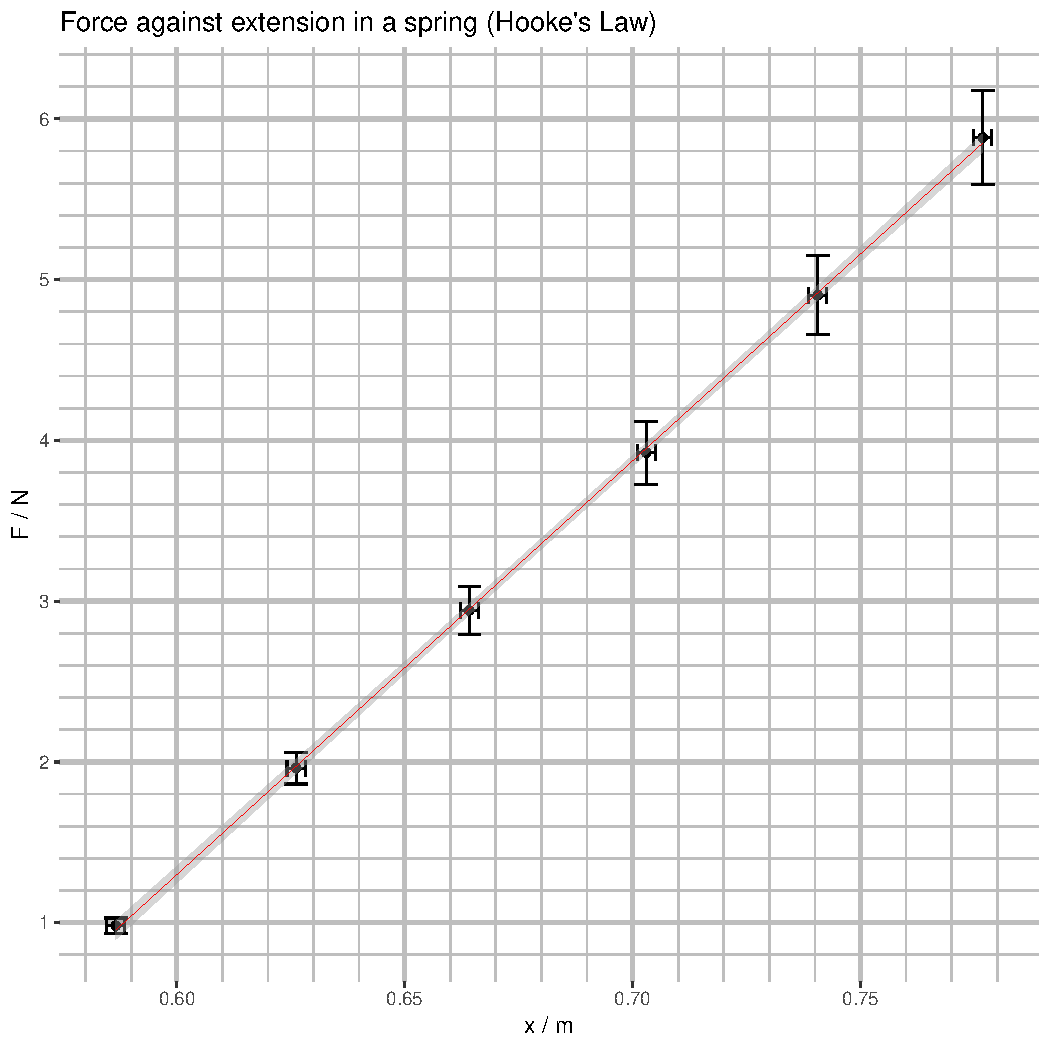
\includegraphics[width=\textwidth,page=1]{Rplots.pdf}
\caption{Static analysis: Graph of $F/\si{\newton}$ against $x/\si{\metre}$}
\label{fig:static}
\end{figure}

\begin{figure}[H]
\includegraphics[width=\textwidth,page=2]{Rplots.pdf}
\caption{Dynamic analysis: Graph of $\omega^2/\si{\hertz^2}$ against
         $\si{\kilogram}/m$}
\label{fig:dynamic}
\end{figure}

This uses the linearisation from
$\displaystyle\omega^2 = \frac km \Rightarrow
    \left(\frac{2\pi}{T}\right)^2 = \left(\frac 1m\right) k$

The linear regression in figure \ref{fig:static} calculated
$k \pm \sigma_{est}$ as \SI{25.7442 \pm 0.1742}{\newton \per \metre}.

The linear regression in figure \ref{fig:dynamic} calculated
$k \pm \sigma_{est}$ as \SI{24.0070 \pm 0.1289}{\newton \per \metre}.

This discrepancy can most likely be explained by the fact that when the spring
was oscillating, the stand was also oscillating, probably causing some kind of
damping.

I'm inclined to prefer the static experiment (Graph \ref{fig:static}), as the
uncertainty remains globally quite low and it produces data that it's easier to
fit a line to (even after linearisation), while not introducing any systematic
error from air resistance or shaking apparatus.

\end{document}
